\chapter{Cluster physics}\label{clustertheo}
In the following we want to review some basic theoretical and observational
facts of cluster physics. The presentation in this section has been inspired by
\citet{Pfrommer2005}, \citet{Sarazin1988}, \citet{Voit2005} and
\citet{Plionis2008}.

\section{Cluster formation}
\subsection{Initial density fluctuations}
On very large scales the universe appears homogeneous and isotropic. However
the existence of stars, galaxies and galaxy clusters demonstrates, that the
universe is not perfectly homogeneous. The early universe must have been
slightly clumpy. These perturbations away from the mean density $\fil{\rho}$ can
be characterized as a overdensity field 
\begin{align}
\delta(\vec{x}) = \frac{\rho(\vec{x})-\fil{\rho}}{\fil{\rho}}
\end{align}
with Fourier transform
\begin{align}
\delta(\vec{k}) = =\ffft\iiiinf \delta(\vec{x}) e^{-i\vec{k}\vec{x}} dV.
\end{align}
In case that $\delta(\vec{x})$ is isotropic, it can be specified by an
isotropic power spectrum
\begin{align}
P(k) = \delta^*(k)\delta(k)= \abs{\delta(k)}^2.
\end{align}
If we assume, that the power spectrum has a power-law form $P(k) \sim k^n$, one
can show \citep{Peebles1970}, that the gravitational potential fluctuations 
$\delta\Phi$ scale as
\begin{align}
\delta\Phi \sim k^{(n-1)/2}.
\end{align}
Therefore the magnitude of these fluctuations diverges on either the
small scale or the high scale end, except in the case of $n=1$. This special
property makes $P(k) \sim k$ the most natural power-law spectrum and it also
appears to be a good approximation to the true power spectrum of density
fluctuations in the early universe. 
\subsection{Hierarchical growth of density fluctuations}
Once the universe has been seeded with density perturbations, they begin to
grow, because the gravity of the overdense regions attracts matter
away from neighboring underdense regions. The gravitational pull of the density
perturbations on the smallest scales causes them to collapse first,
because, as shown in the last section, the density perturbations have larger
amplitude on smaller mass scales. That's why the standard model of cosmology
envisions structure formation as a hierarchical process in which gravity is
drawing matter together to form increasingly larger structures.
Clusters of galaxies are believed to be the largest structures formed by this
process nowadays. Since it is assumed in the standard model, that most
of the matter in the universe is cold, collisionless dark matter\footnote{The
evolution of cold, collisionless dark matter can be described by the
Vlasov-Poisson system of equations, see appendix \ref{vlaspois}.}, the evolution
of clusters is basically governed by the collisionless build-up of dark
matter from small to successively larger haloes. In the
course of this
evolution, small structures merge to form larger structures. A full
understanding of this hierarchical merging process requires
numerical simulations, although its basic concepts can be obtained by means of
the analytical spherical collapse model \citep{Gunn1972,Bertschinger1985}.

However, the accretion process in real clusters is not symmetric. Gravitational
forces between merging matter clumps produce a time-varying collective
potential which randomizes the velocities of the infalling particles yielding
a Maxwellian velocity distribution. This process is known as violent relaxation
\citep{Lynden-Bell1967} and leads to a state of virial equilibrium.
The final outcome of such a virialized, collisionless system would be a
self-gravitating isothermal sphere, in which the velocity dispersion $\sigma_v$
is constant and isotropic at every point and the density profile is
\begin{align}
\rho(r)= \frac{\sigma_v^2}{2 \pi G r^2}.
\end{align}
But this model leads to the unfortunate result of infinite mass and energy
for a galaxy cluster, and so it can never exist in nature.

Numerical N-body simulations instead find that the profile of dark matter halos
is described by a universal law \citep{Navarro1997}
\begin{align}
\rho_{dm}(r)=\frac{\rho_{dm,0}}{r(r+r_0)^2},\label{eq:NFW}
\end{align}
where $\rho_0$ is the central density and $r_0$ a characteristic scale
radius.
But even with this more sophisticated density profile mass diverges
logarithmically with radius. Thus, the cluster’s mass and
relations linking that mass to observables depend crucially on the definition of
the outer boundary of the cluster. It turns out, that their is no unique
definition for the boundary of a cluster, however a common definition, also used
in the analysis tools for this work, is the scale radius $r_{200}$ within which
the mean matter density is 200 times the critical density 
$\rho_{cr}=\frac{3H(z)^2}{8\pi G}$ of the universe \footnote{Although not
precicely equivalent, we will call $r_{200}$ the virial radius and
the mass inside this radius the virial mass in our work.}. 

\section{Intracluster medium}
It is widely assumed, that the total matter density profile of the galaxy
clusters follows the NFW dark matter profile (equation \eqref{eq:NFW}),
because the dark matter accounts for the biggest part of the total mass.
The profile of the baryonic density will also follow the NFW profile on
the larger scales, because the baryons follow the gravitational potential of
the dark matter. Only in the core, significant deviations from the NFW profile
can be expected for the baryonic density, since the baryons are not
collisionless and pressure effects should lead to a different profile.
This can be tested by measurements of the extended x-ray emissions of the
intracluster medium and by numerical fluid dynamical simulations, if the mean
free path of the very hot, but dilute ICM is small enough.  
\subsection{Mean free path of the ICM}\label{mfp}
To check, if the fluid assumption holds for the ICM, it is
important to estimate the mean free path. The mean free path of electrons and
protons in a plasma is determined by coulomb collisions. The electrons in a
Maxwellian plasma undergo Coulomb collisions in a time which is a factor of
$\sim \sqrt{m_e/m_p}$ shorter than the protons. On the other hand, the electrons
move faster by the inverse of this factor. Thus, the mean free paths of
electrons and protons are essentially equal, with \citep{Plionis2008}
\begin{align}
\lambda_e=\lambda_p \approx 23 
\lra{\frac{T}{\unit[10^8]{K}}}^2 
\lra{\frac{n_e}{\unit[10^{-3}]{cm^{-3}}}}^{-1} \unit{kpc}.
\end{align}
So for typical values of temperature and density of the ICM, we have mean free
paths of the order of $\unit[10]{kpc}$, which is roughly the scale of a galaxy.

However the ICM contains a significant magnetic field \citep{Plionis2008}, with
typical values of $B=\unit[1]{\mu G}$, which might be not dynamically relevant
on large scales, but it alters the microscopic motions of the electrons and
protons. In a magnetic field, charged particles follow helical orbits, gyrating
about magnetic field lines. For example the gyroradius of a typical electron is 
\begin{align}
r_g \approx 9.72 \cdot 10^{-11} 
\lra{\frac{T}{\unit[10^8]{K}}}^{1/2} 
\lra{\frac{B}{\unit[1]{\mu G}}} \unit{kpc}. 
\end{align}
These very small gyroradii probably ensure that the ICM acts as a fluid even
when the Coulomb mean free paths are long. 

\subsection{Magnetic fields}
The general consensus is, that no mechanism can produce significant magnetic
fields in the ICM prior to the formation of galaxies and large scale structures
\citep{Kulsrud2008}. So where do the significant magnetic fields in the ICM
mentioned in chapter \ref{mfp} come from? It is assumed, that weak seed fields
were created early in the universe by the so called Biermann battery mechanism
\citep{Biermann1951}, which predicts fields of a strength $\approx
\unit[10^{-20}]{G}$. Several theories (e.g. \citet{Kulsrud1992})
expect that these seed fields were amplified by Kolmogorov turbulence by a
factor of $10^{14}-10^{15}$, which yields a magnetic field strength of 
$\approx \unit[1]{\mu G}$ nowadays, a value which is observationally found in
cores of galaxy clusters \citep{Carilli2002}. 

But what is the driving mechanism, which generates the turbulence amplifying
the magnetic field in cluster cores? One process are merger events. 
\citet{Roettiger1999}
found, that the field energy after a merger is found to increase by nearly a
factor of three (and locally up to a factor of 20) with respect to a non-merging
cluster. Since it is quite likely, that a galaxy cluster experiences more than
one of these events, the amplification will be even larger. Nevertheless the
most significant process one can think of is the Kelvin-Helmholtz (KH)
instability driven by shear flows, which are common during the formation of
cosmic structures. When applied to a cluster core enviroment, the core
dimensions basically define 
the injection scale and the KH timescale turns out to be $\unit[10^7]{years}$,
which makes this instability an interesting process to amplify weak magnetic
fields \citep{Dolag2008}. 

However although numerical simulations could show, that the amplification of
magnetic fields by shear flows is significant
\citep{Dolag2005a,Bruggen2005}, they still have problems explaining the large
amplification factors of the initial magnetic fields. \citet{Dolag2005a}, who
used a Magnetic Smoothed Particle Hydrodynamic code, had to assume a initial
seed field of $\unit[10^{-11}]{G}$ at a redshift $z=20$ to achieve realistic
magnetic field strengths at $z=0$. But these problems might be due to the
numerical method used. Only recently it has been shown by \citet{Agertz2007},
that Smoothed Particle Hydrodynamic (SPH) codes have severe problems describing
Kelvin-Helmholtz instabilities. Although a solution to these problems has
already been proposed by \citet{Price2007}, we have to assume, that up
to now basically all SPH simulations of turbulence driven by flow instabilities
are questionable. Hence a better treatment of turbulence is necessary to
be able to study the evolution of magnetic fields in galaxy clusters. 

\subsection{X-ray observations of the ICM}
X-ray observations are the most accurate source of information about galaxy
clusters today. Observables in the X-ray band include the overall X-ray
luminosity of a cluster, emitted by the hot plasma trapped
in the cluster’s gravitational potential and the cluster’s temperature inferred
from the X-ray spectrum of that plasma. From these data, one can reconstruct
density, temperature and entropy profiles. Of course, projection effects,
cluster substructure, and deviations from spherical symmetry complicate the
generation of these profiles. However only recently \citet{Nagai2007}
could demonstrate using data from cosmological simulations, that the methods
used by \citet{Vikhlinin2006} for analyzing X-ray data of the the
X-ray satellite CHANDRA, can reliably recover the distribution of density and
temperature of the hot ICM.  So given these three-dimensional models for the gas
density and temperature profiles, the total gravitational mass within the radius
$r$ can be estimated from the hydrostatic equilibrium equation in the
form\footnote{For a derivation see appendix \ref{stat}.} 
\begin{align}
M(r) &= - \frac{R_s T_g r}{G} \lra{\ppd{\ln r}{\ln T_g}+\ppd{\ln r}{\ln
\rho_g}}.
\end{align}
Given $M(r)$, one can then calculate the total
matter density profile
\begin{align}
\rho(r)=\frac{1}{4\pi r^2} \ttd{r}{M}. 
\end{align}
The result of such an analysis \citep{Vikhlinin2006} can be seen in figure
\ref{fig:profiles}. 
\begin{figure}[tp]
	\centering
	\subfigure[Density profiles for gas density $\rho_{gas}$ and total density 
	$\rho_{tot}$.]
	{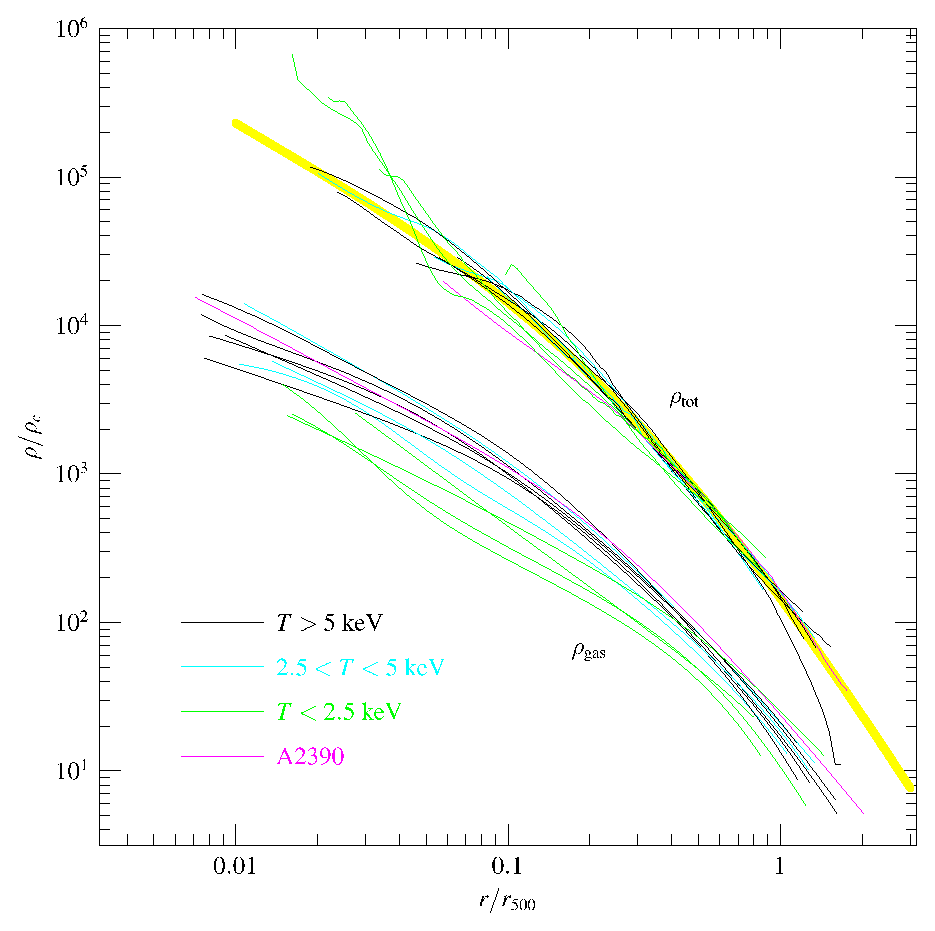
\includegraphics[width=0.6\linewidth]{cluster/rhoprof.eps}}
	\subfigure[Temperature profiles.]
	{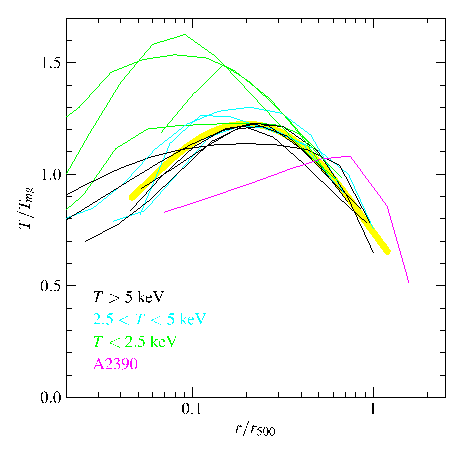
\includegraphics[width=0.6\linewidth]{cluster/Tprof.eps}}
	\caption{Scaled density and temperature profiles for galaxy clusters
	observed with CHANDRA by \citep{Vikhlinin2006}. The yellow line are a NFW
	fit to the total gas density and a average fit to the temperature profiles.}
	\label{fig:profiles}
\end{figure}
It is apparent, that the NFW profile provides a good fit for the density
profile of the total mass of the clusters. The scatter in the baryonic density 
profiles is significantely larger and for lower temperature clusters the
profiles are flatter towards the center of the cluster. The temperature
profiles also show signs of self-similarity, at least for the higher
temperature clusters $T > \unit[2.5]{keV}$, which are fitted by
\begin{align}
\frac{T(r)}{T_{mg}} = 1.35 \frac{(x/0.045)^{1.9} + 0.45}{(x/0.045)^{1.9}+1}
\frac{1}{\lrb{1+(x/0.6)^2}} 
\end{align}
where $x=r/r_{500}$ according to \citep{Vikhlinin2006}. Also visible from the
temperature fit are a isothermal plateau at $r \approx \unit[0.2]{r_{500}}$ and
the significant decrease of temperature towards the center. This behavior is
often
explained by assuming some cooling mechanism. Theoretically cooling
should lead to lower pressure in the center of the cluster, thereby leading to
an even denser core to maintain hydrostatic equilibrium. But, because cooling is
even more effective at lower densities, this process is instable leading to
catastrophic cooling of the core, which is not observed, giving rise to the
so called "cluster cooling flow problem". Observationally emissions from the
central cluster gas can be detected for gas temperatures between the ambient
temperature $T_0$ and $\sim T_0/2$, but not below $<T_0/3$ \citep{Peterson2003},
so some sort of heating mechanism seems to be inhibiting the cooling below this 
temperature. There are plenty of candidates for this - supernovae, outflows
from active galactic nuclei, thermal conduction and turbulent mixing - but
there is still no consensus on the relative importance of these mechanisms.
Turbulence is especially interesting, because it was also
suggested by \citet{Nagai2007} as mechanism, which might explain some
deviations in the computation of the total mass,
which is based on the assumption of hydrostatic equilibrium, without taken
turbulent pressure into account. 

\subsection{Turbulence in the ICM}
The "bottom-up" model or hierarchical model of cosmological structure formation
\citep[eg.,][]{Ostriker1993} explains the build up of clusters through a
sequence of mergers of lower-mass systems (stars $\rightarrow$ galaxies
$\rightarrow$ groups $\rightarrow$ clusters). In particular, mergers of galaxies
play a fundamental role in 
determining the structure and dynamics of massive clusters of galaxies. It is
found that major mergers induce temperature inhomogeneities and bulk motions
with velocities $> \unit[1000]{km\ s^{-1}}$ in the intracluster medium (ICM)
\citep{Norman1999a}. This results in complex hydrodynamic flows where most of
the kinetic energy is quickly dissipated to heat by shocks, but some part may in
principle also excite long-lasting turbulent gas motions.

In numerical simulations of merging clusters \citep{Schindler1993, 
Roettiger1997,Ricker2001,Takizawa2005} it has been shown, that infalling
subclusters generate a laminar bulk flow, but inject turbulent motions via
Kelvin-Helmholtz instabilities at the interfaces between the bulk flows and the
primary cluster gas. Such eddies redistribute the energy of the merger through
the cluster volume and decay with time into more and more random and turbulent
velocity fields, eventually developing a turbulent cascade with a spectrum of
fluctuations expected to be close to a Kolmogorov spectrum \citep{Dolag2005}. 

The turbulent nature of the flow could be directly confirmed with the help of
high-resolution X-ray spectroscopy of emission line broadening of lines of
heavy ions. It has been suggested \citep{Sunyaev2003}, that the X-ray
microcalorimeters (XRS) on board of the X-ray satellite ASTRO-E2\footnote{Also
called \emph{Suzaku}.} should be able to detect this broadening. But due to a
critical flaw in the XRS instrument in August 2005, this test has to be
postponed until future instruments like XEUS are available. Nevertheless other
observations have revealed some signature for turbulence in the ICM.
For example \citet{Schuecker2004} analyzed the pressure
fluctuation spectrum of the Coma cluster claiming that it scales according to
Kolmogorov-Obukhov theory (see figure \ref{fig:schuecker}).

\begin{figure}[tp]
\centering
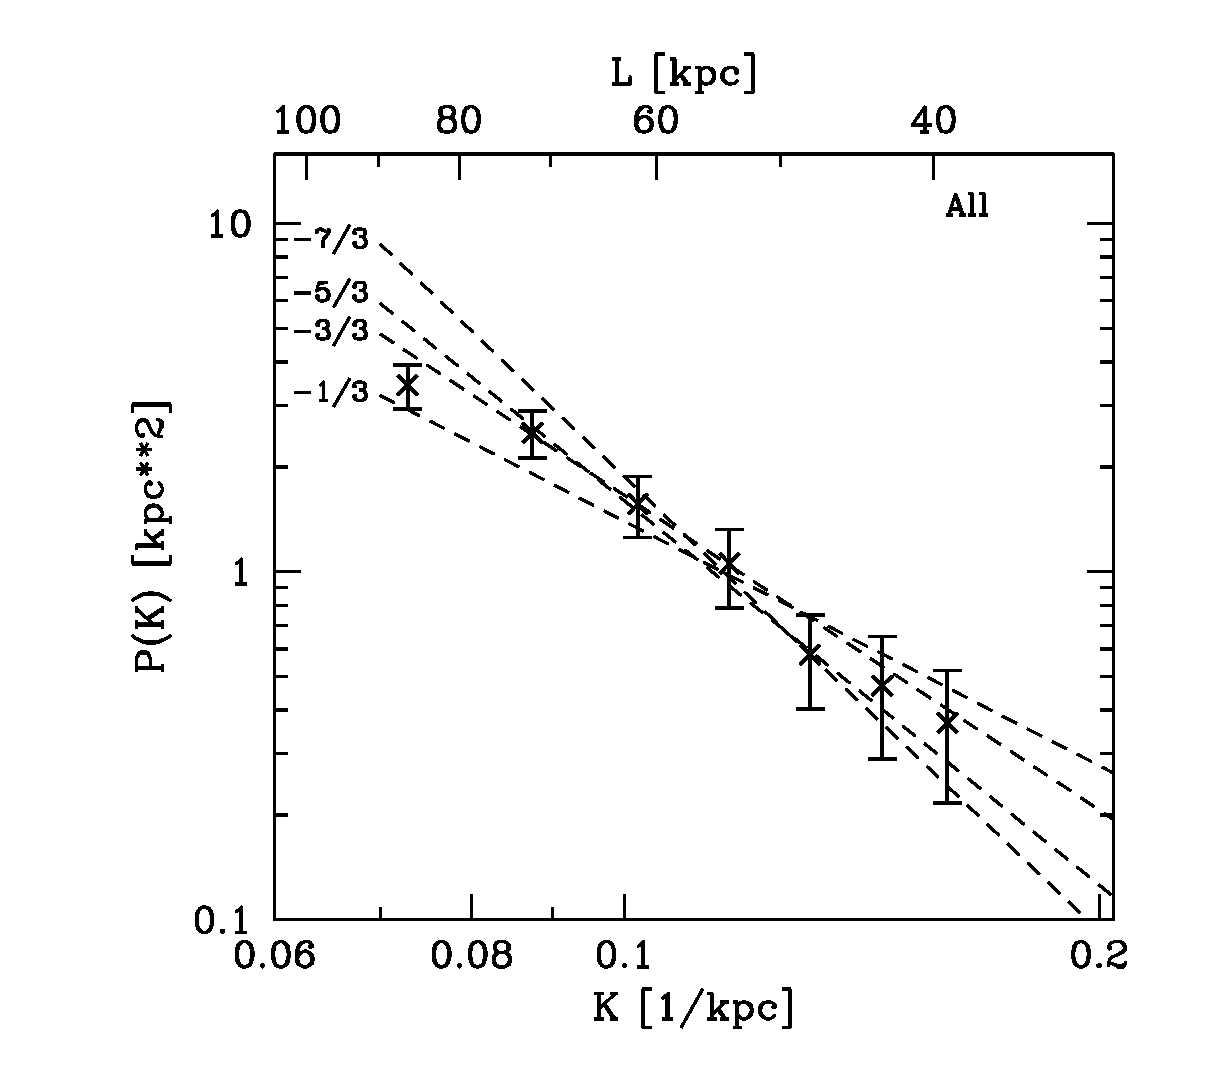
\includegraphics[width=0.7\linewidth]{chapter8/1039fg12.eps}
\caption{Observed projected shot-noise-subtracted 
power spectral densities (dots with $1\sigma$ error bars) compared with model
predictions (dashed lines). From \citet{Schuecker2004}.}
\label{fig:schuecker}
\end{figure}
\begin{figure}[tp]
\centering
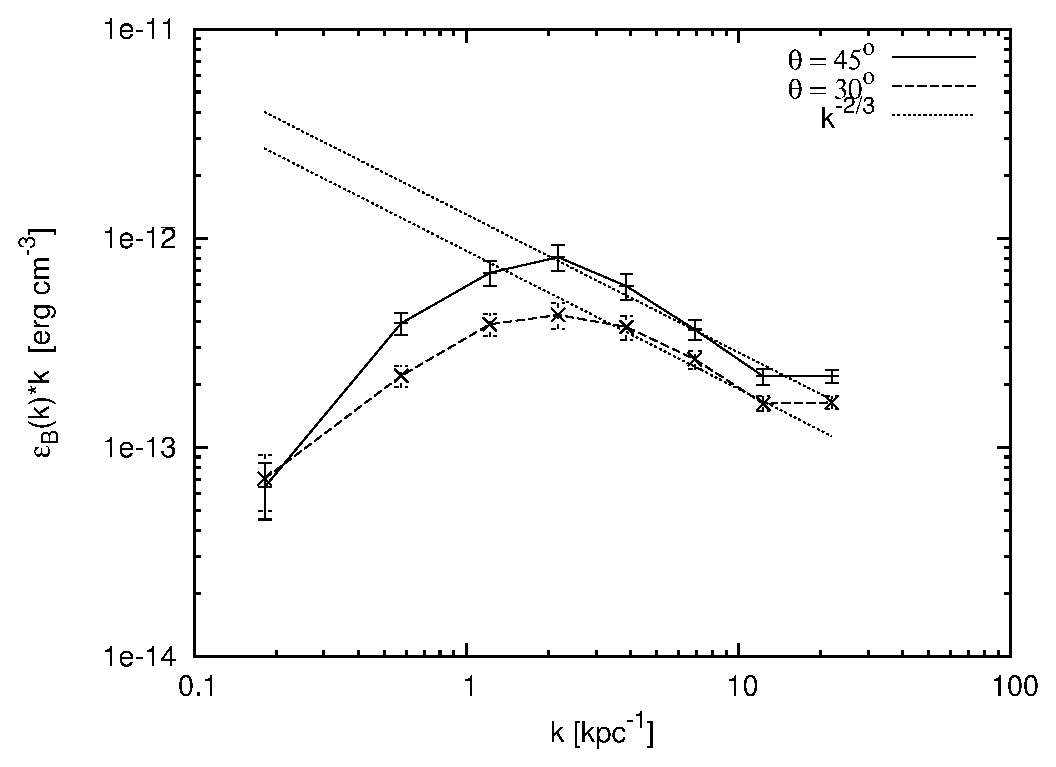
\includegraphics[width=0.7\linewidth]{chapter8/fig7.eps}
\caption{Power spectra for two different
inclination angles $\theta = 30^\circ$ and $\theta = 45^\circ$.
For comparison a Kolmogorov-like power spectrum is
plotted as a straight dashed line. One can see that the calculated
power spectra follow such a power spectrum over at least one order of
magnitude. From \citet{Vogt2005}.}
\label{fig:vogt}
\end{figure}

\citet{Vogt2005} makes
use of the Faraday rotation effect to investigate the magnetic field structure
of the ICM in the Hydra cluster. They extract magnetic field strength power
spectra from their data and find a Kolmogorov scaling behavior below a
length scale of \unit[1]{kpc} (see figure \ref{fig:vogt}) . 

Furthermore the broadening of the iron abundance profile
in the core of the Perseus cluster \citep{Rebusco2005} and other galaxy
clusters \citep{Rebusco2006} and the lack of 
resonant scattering in the $\unit[6.7]{keV}$ He-like iron K$_{\alpha}$ line in
the Perseus cluster \citep{Churazov2004} can also be interpreted as evidence for
the turbulent state of the ICM. 


 

 
